\documentclass[12pt,a4paper]{article}

\usepackage[slovak]{babel}
\usepackage[T1]{fontenc}
\usepackage[utf8]{inputenc}
\usepackage[left=2.5cm, right=2.5cm, top=3cm, bottom=3cm]{geometry}
\usepackage{booktabs}
\usepackage{tabularx}
\usepackage{fancyhdr}
\usepackage{parskip}
\usepackage{hyperref}
\usepackage{float}
\usepackage{graphicx}

\linespread{1.3}

\hypersetup{colorlinks=true, linkcolor=black, urlcolor=black, citecolor=black}

\pagestyle{fancy}
\fancyhf{}
\rhead{\small AutoBook~·~Zadanie 2 Checkpoint}
\lhead{\small OOP~·~2025/2026}
\cfoot{\small\thepage}
\renewcommand{\headrulewidth}{0.4pt}

\begin{document}

\begin{titlepage}
\centering

\vspace*{3cm}

{\Huge\textbf{AutoBook}}

\vspace{0.4cm}
\rule{8cm}{0.8pt}
\vspace{0.4cm}

{\large Zadanie 2~·~Checkpoint Dokumentácia}


\vspace{3cm}

\begin{tabular}{cc}
\centering\large\textbf{Andrii Dosyn} & \centering\large\textbf{Anton Hrimov}
\end{tabular}

\vspace{3cm}

\end{titlepage}

\tableofcontents
\newpage

\section{Špecifikácia zadania a Zámer}

AutoBook je platforma fungujúca pre autorov a čitateľov. Spája komunitu ľudí a poskytuje inteligentný analytický nástroj pre autorov -- \textbf{Vocabulary Builder} -- s podporou umelej inteligencie (NLP). Projekt bol rozvrstvený na hlavnú Java Spring Boot aplikáciu a Python FastAPI mikroslužbu zodpovednú za analytiku.

\textbf{Hlavné funkcionality pre Checkpoint (základná implementácia):}
\begin{itemize}
    \item Používateľský systém, publikovanie kníh a písanie príspevkov v rámci kompozytnej hierarchie z backend prístupu.
    \item Interakcia formou komentárov a sledovania (\textit{Follow}) autorov.
    \item Generovanie slovníka (Vocabulary).
    \item Služby implementované primárne v Jave nad databázou, prepájajúce entitné formáty pomocou JPA.
\end{itemize}

\section{Deklarácia použitých OOP princípov}

Zdrojový kód systému bol navrhnutý podľa princípov objektovo-orientovaného programovania, s dôrazom na oddelenie logiky a vrstiev dát.

\subsection{Generalizácia (Generalization)}
Uplatnili sme princíp generalizácie tak pri konšturkcii rozhraní, ako aj v Java výnimkách. Dobrým príkladom je dedenie vlastných výnimiek od všeobecného typu \texttt{RuntimeException}, alebo využívanie všeobecného abstraktného typu v AI prístupe k úložisku. Kód ukazuje generalizovaný pohľad na odchytávanie chýb priamo v business vrstve aplikácie (\texttt{Exception} balík v Jave).

\begin{figure}[H]
\centering
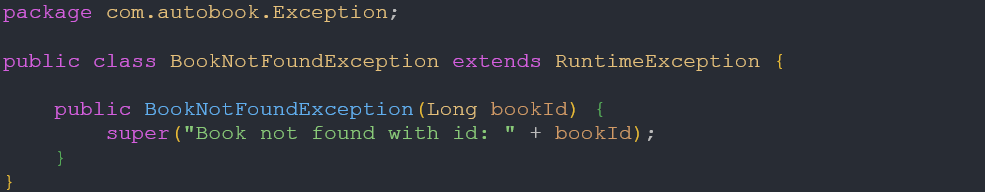
\includegraphics[scale=0.6]{f1.png} 
\end{figure}

\subsection{Agregácia (Aggregation)}
V Java entitách sme nastavili agregáciu prostredníctvom voľných kompozitných väzieb. Napríklad rola \textbf{Autora} a \textbf{Knihy} v balíku `com.autobook.Library.Book.Book`. Kniha uchováva objekt `User` (autora) pomocou anotácie rozhrania `@ManyToOne`. Používateľ bez nej dokáže nezávisle naďalej existovať a uplatňovať svoju entitnú logiku inde na sieti a v príspevkoch.

\begin{figure}[H]
\centering
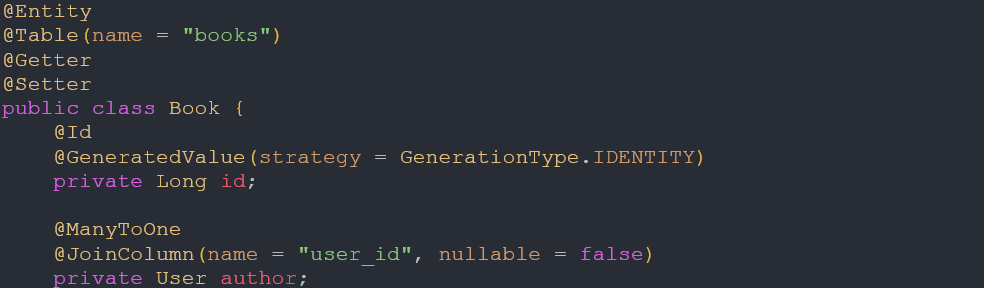
\includegraphics[scale=0.6]{f2.png} 
\end{figure}

\subsection{Kompozícia (Composition)}
Silnú väzbu s plným riadením životného cyklu demonštruje vzťah \textbf{Post} a \textbf{Comment}. Komentáre sú existenčne viazané na príspevok pod ktorým visia. V entitnom kóde \texttt{Post.java} je použitá kaskáda typu \texttt{CascadeType.ALL} a parameter \texttt{orphanRemoval = true}, čo fyzicky vynucuje OOP kompozíciu brániacu úniku dát z pamäte.

\begin{figure}[H]
\centering
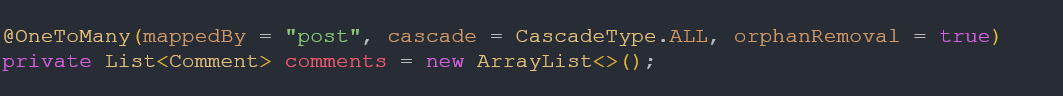
\includegraphics[scale=0.6]{f3.png} 
\end{figure}

\subsection{Dedenie: Dve hierarchie (Inheritance)}
Projekt striktne uplatňuje systém kódovania do hierarchií, aby sme zachovali rozšíriteľnosť pre budúcnosť. Uplatňujeme nasledovné dve preukázateľné dedičné cesty:

\textbf{1. Hierarchia v dátovom formáte (\textit{Python mikroslužba})} \\
Úložisko tvorené rodičom `BaseStorage` určujúcim zmluvný kontrakt dovoľuje poddediť triedy implementátorov pre databázu `MongoStorage` a lokálne úložisko pre disky `FileStorage`.
\begin{figure}[H]
\centering
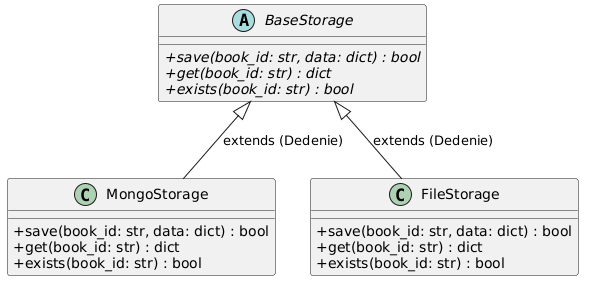
\includegraphics[scale=0.5]{diagram_storage_python.png} 
\caption{Dedenie prvej hierarchie: Polymorfné abstraktné úložisko.}
\end{figure}

\begin{figure}[H]
\centering
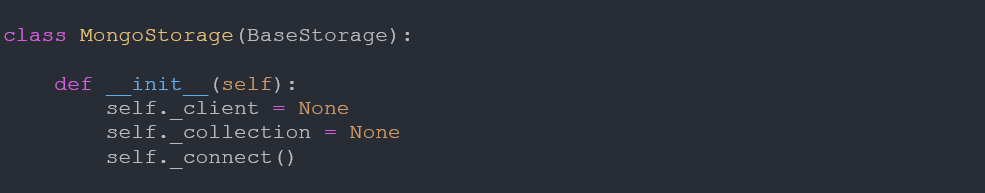
\includegraphics[scale=0.6]{f4.png} 
\end{figure}

\textbf{2. Hierarchia chýb (\textit{Java Autorské Výnimky})} \\
Druhú dedičnú vetvu reprezentuje balík s výnimkami. Každé porušenie biznis logiky (neexistencia knihy, používateľa, zlé id) prediedla priamo z nadradenej java triedy \texttt{RuntimeException}.
\begin{figure}[H]
\centering
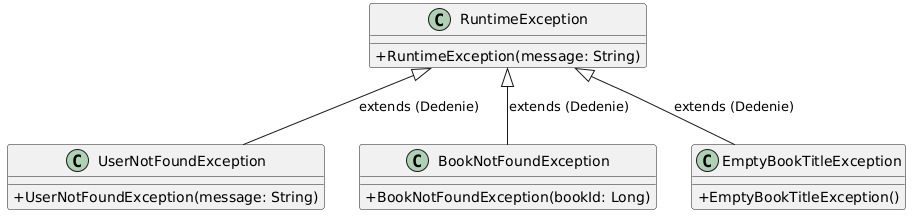
\includegraphics[scale=0.5]{diagram_exception_java.png} 
\caption{Dedenie druhej hierarchie: Hierarchia Java výnimiek \texttt{RuntimeException}.}
\end{figure}

\begin{figure}[H]
\centering
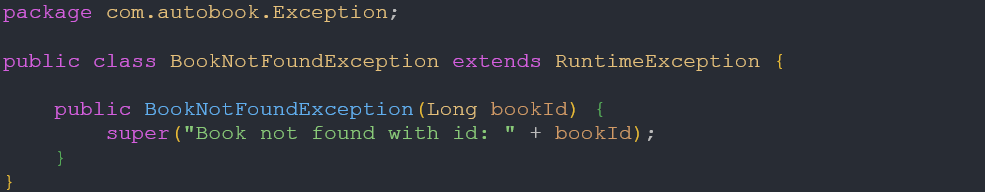
\includegraphics[scale=0.6]{f1.png} 
\end{figure}

\newpage

\subsection{Polymorfizmus (Compile-time a Run-time)}

\textbf{Polymorfizmus za behu (Run-time overriding):} \\
Uplatnený najviac pri prístupoch nad úložiskom v Python mikroservise, kde samotná analytická logika poberá v úvode polymorfný dcérový objekt (napr. \texttt{MongoStorage}), no posiela mu dopyt nad fasádou abstraktnej volajúcej metódy rodiča z inštancie `BaseStorage`. 

\textbf{Polymorfizmus pri preklade (Compile-time overloading):} \\
Typicky prítomný na repozitárnych dopytoch s dynamickým \textit{overloadingom} pri preťažení. Napríklad dopyty \texttt{findByAuthor(User author)} vs. \texttt{findByAuthorAndPrivacy(User author, PrivacyType privacy)} v \texttt{BookService.java} simulujú zmenený signatúrny model vyhľadávania nad knihami v jedinom kontexte preťaženia rovnakého požiadavku.

\begin{figure}[H]
\centering
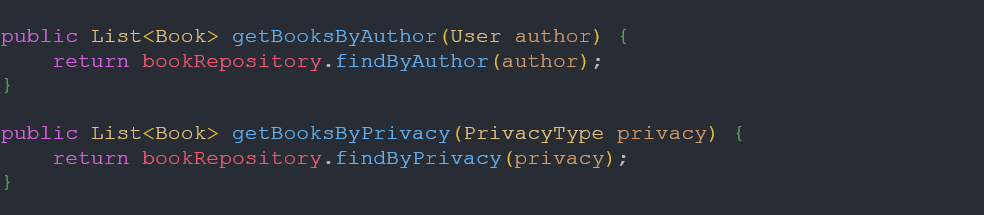
\includegraphics[scale=0.6]{f5.png} 
\end{figure}

\subsection{Preťaženie (Overloading)}
Preťažovanie doménových konštruktorov v javovskej knižnici výnimok. Napríklad vyvolanie inštancie z \texttt{RuntimeException(String)} namiesto prázdnej konštrukcie obohacuje stav objektu metódami poslenými počas kompilácie. Toto generuje konštrukcie obalov na chybové javy.

\begin{figure}[H]
\centering
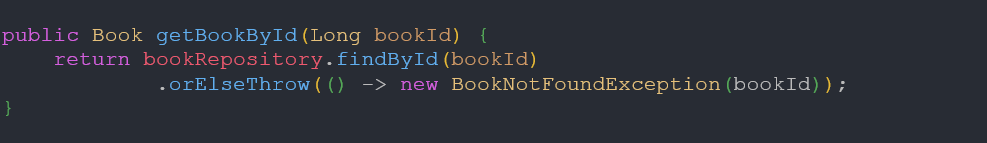
\includegraphics[scale=0.6]{f6.png} 
\end{figure}

\subsection{Prekonanie (Overriding)}
Použitie a priame dedičné prekonávanie metód realizujeme v abstraktnej databáze `BaseStorage.save()` (v Pythone cez `@abstractmethod`), ktorej implementačný prístup \texttt{MongoStorage} povinne realizuje (\texttt{Overriding} správania). V Jave samotné výnimky prepisujú svoj stavový výpis chýb posúvaním chybovej inštancie priamo do rodicovskej triedy (výpis `super(msg)`).

\begin{figure}[H]
\centering
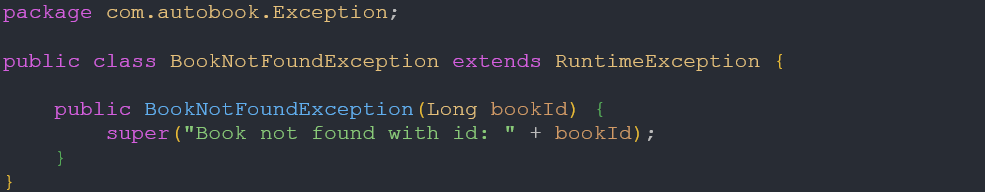
\includegraphics[scale=0.6]{f1.png} 
\end{figure}

\section{Diagram tried entít}

Dátová a logická previazanosť základnej doménovej vrstvy aplikácie v Jave zahŕňa modely užívateľov, publikácií, komentárov, označení a žiadostí na editáciu.
\begin{figure}[H]
\centering
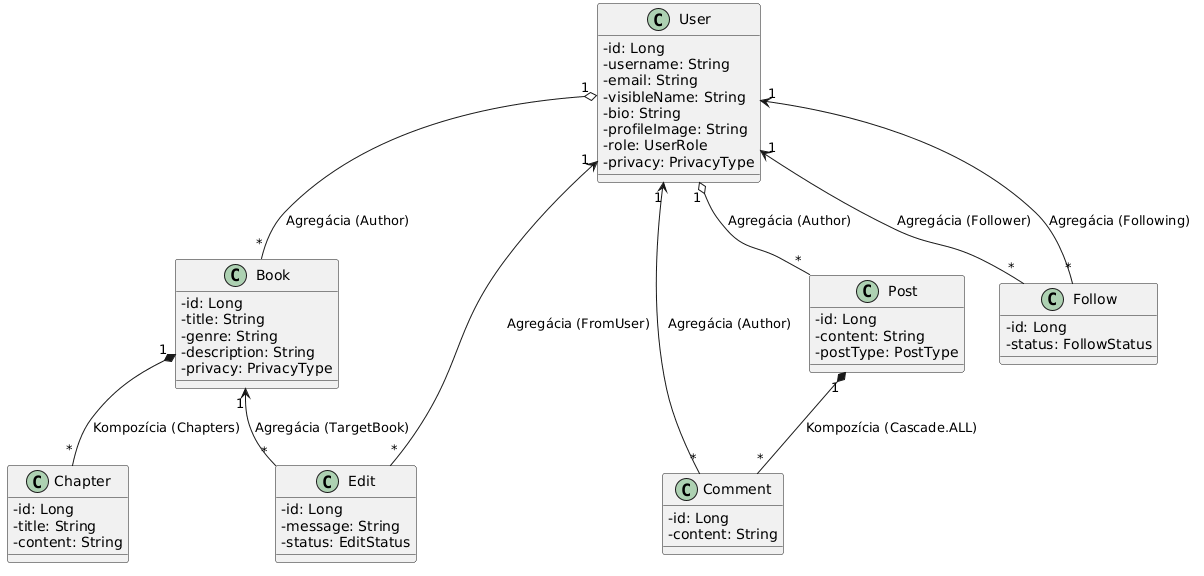
\includegraphics[width=1.0\textwidth]{diagram_entity_java.png}
\caption{Kompletný diagram zdôrazňujúci asociácie, agregáciu a krížovú kompozíciu repozitárnych Java entít.}
\end{figure}

\section{AI Mikroslužba}

AutoBook AI je samostatný mikroservis zameraný na analýzu textu pomocou metód spracovania prirodzeného jazyka (NLP). Slúži ako inteligentné \textbf{analytické jadro} platformy. Z decentralizácie vyplýva uvoľnenie záťaže hlavnej Java (Spring Boot) aplikácie.

\subsection{Architektúra a storage mikroservisu}
Aplikácia je postavená ako REST API pomocou asynchrónneho frameworku \textbf{FastAPI} v jazyku \textbf{Python}. Python bol zvolený pre výborný komunitný prístup k NLP knižniciam:
\begin{itemize}
    \item \textbf{spaCy} -- Zabezpečuje lemmatizáciu a hľadanie štrukturálnych autorských fráz v angličtine.
    \item \textbf{TextBlob} -- Vyhodnocuje "sentiment" (emócie a subjektivitu vetnej stavby kapitol).
\end{itemize}

O ukladanie stavov sa stará dokumentová vrstva nad \textbf{MongoDB}, čím dokážeme zachovať polia metrík s variabilnou JSON dĺžkou. Ako úložisko pre vývoj slúži \textit{File Storage}.

\begin{figure}[H]
\centering
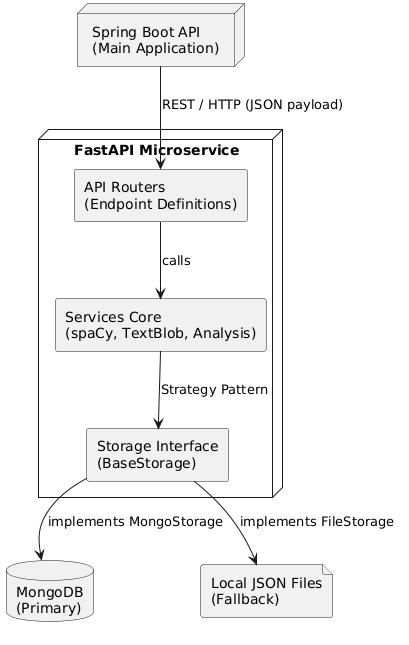
\includegraphics[width=0.4\textwidth]{diagram_arch_ai.png} 
\caption{Decentralizovaná architektúra mikroslužby zaťaženej AI operáciami.}
\end{figure}

\subsection{Zapuzdrenie (Encapsulation)}
Analytické triedy (napr. \texttt{StyleConsistencyAnalyzer}) vo vysokej miere využívajú zapuzdrenie. Komplexná matematika je pre vonkajší kód zakrytá v bezpečných chránených metódach (ako \texttt{\_lexical\_similarity} a \texttt{\_phrase\_coverage}).

\subsection{Princíp jednej zodpovednosti (SRP)}
Architektúra rozdeľuje logiku tak, aby kontrolery pre API dopyty nikdy priamo nerátali analytiku, a naopak analytické enginy nepoznajú vrstvu HTTP zberu dát formou \textit{Routers} $\rightarrow$ \textit{Services} $\rightarrow$ \textit{Models}.

\section{Unit testy a Integrácia}

V súčasnosti je aplikácia dôkladne pokrytá testami pre dôležité služby. Logika \textbf{v Jave} je prítomná v testovacom súbore \texttt{BookServiceTest.java} využívaním \textbf{JUnit 5} a knižnice \textbf{Mockito}. Pokryté je vstrekovanie simulovaných závislostí repozitárnych implementácii ako `InjectMocks` a `Mock`. 

\textbf{Popis kľúčových Unit testov (Java):}
\begin{enumerate}
    \item \textbf{\texttt{createBook\_ok}} a \textbf{\texttt{createBook\_emptyTitle}}: Overujú správanie vytvorenia knižnej publikácie po prijatí správneho obsahu oproti zamietnutiu (vyvolaniu explicitnej výnimky \texttt{EmptyBookTitleException}) v prípade prázdneho názvu. 
    \item \textbf{\texttt{getBookById\_ok}} a \textbf{\texttt{getBookById\_notFound}}: Testujú Optional prístup z databázy. Ak UUID neexistuje, \texttt{assertThrows} potvrdí vyhodenie výnimky \texttt{BookNotFoundException}.
    \item \textbf{\texttt{updateBook\_ok}}: Overuje správanie prikázanej editácie entít so simulovanými zmenami vlastností od klienta.
\end{enumerate}

Súčasné Python scripty v AI analytike sa stavajú formou integračných jednotiek skrz \textbf{pytest}.
\textbf{Popis kľúčových Unit testov (Python):}
\begin{enumerate}
    \item \textbf{\texttt{test\_routes}}: Overuje endpointy FastAPI, správnosť prenosu JSON štruktúr nad aktívnym routerom a testuje HTTP stavové kódy odozvy mikroslužby pri zaslaní analytických textových dopytov.
\end{enumerate}

\section{Implementácia používateľského rozhrania}

Nasledujúce obrazovky predstavujú reálnu funkčnú implementáciu grafického rozhrania (frontend) systému AutoBook. Podrobný manuál ako systém \textit{spustiť} sa nachádza v priloženom \texttt{README.md} v koreni repozitára.

\subsection*{Použité technológie (Frontend stack)}
Rozhranie je plne vyvinuté v \textbf{TypeScripte} pomocou \textbf{React}. Pre štylizáciu bol zvolený plynulý Dark Mode. Aplikácia využíva klientske smerovanie (React Router) a robustný textový editor \textbf{Tiptap}.

\subsection{Hlavná stránka (Feed)}

\begin{figure}[H]
\centering
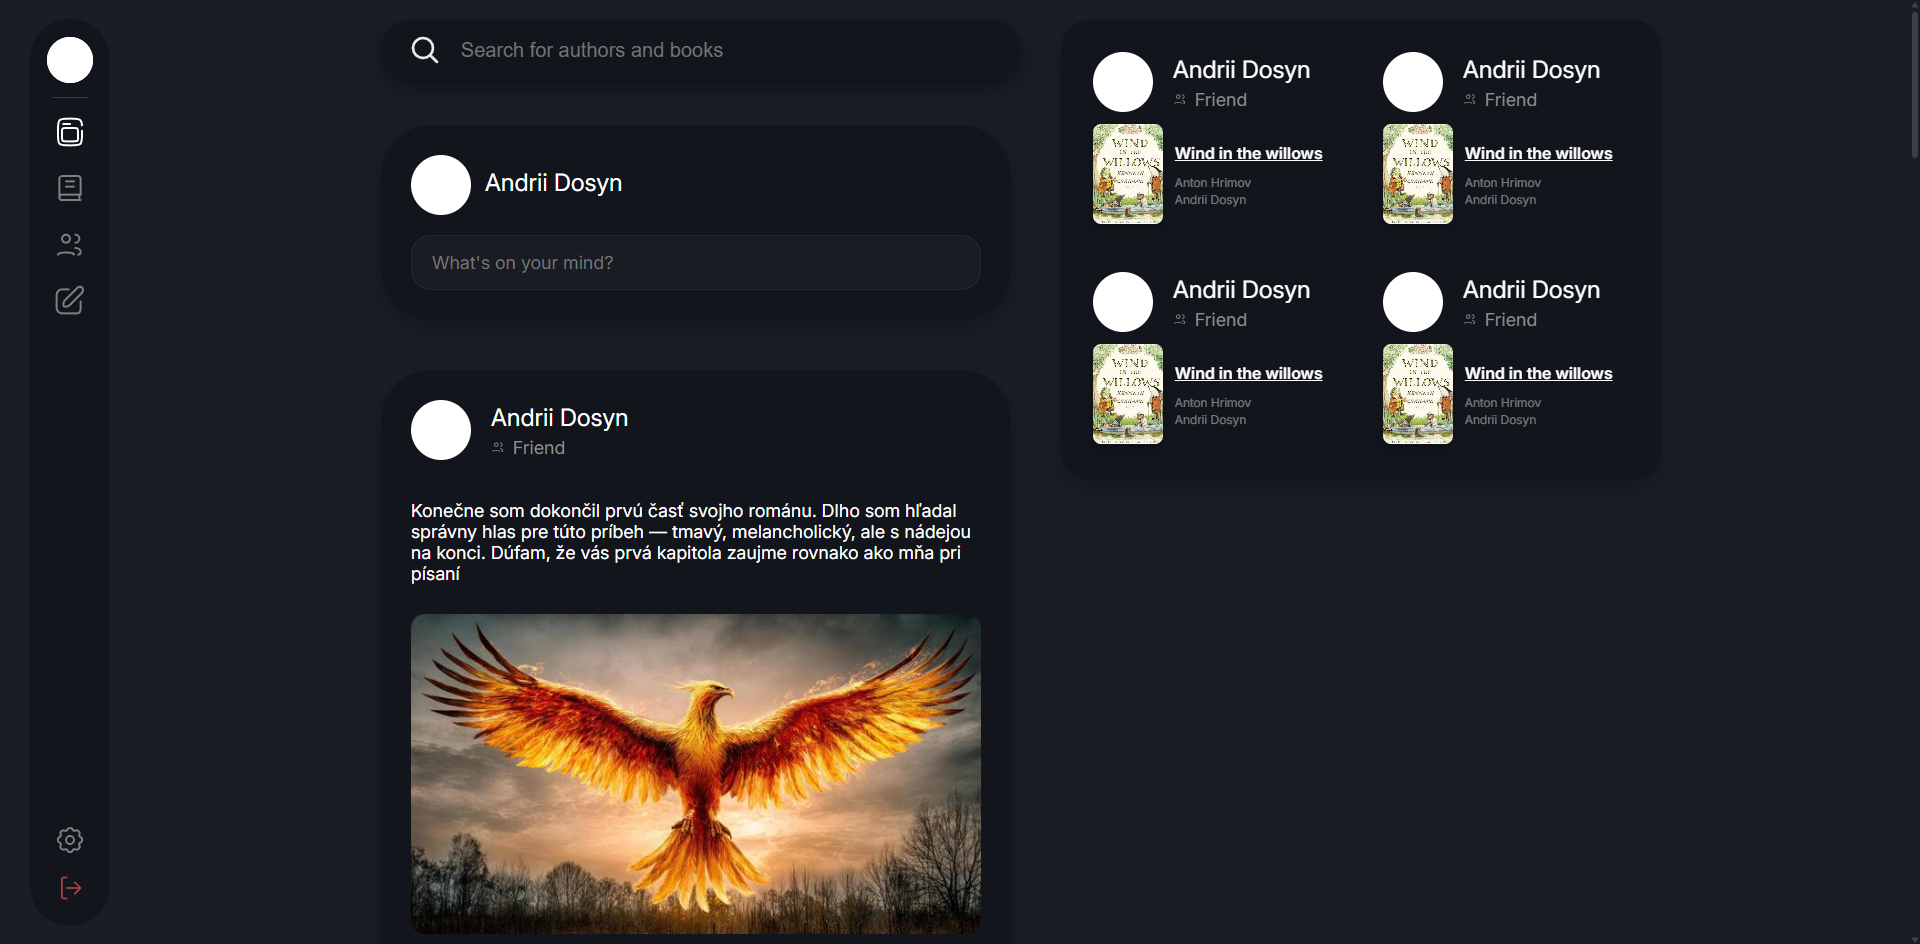
\includegraphics[scale=0.23]{feed.png}
\end{figure}
Hlavná informačná os zobrazujúca aktivitu siete. Ponúka inline formuláre pre sociálne interakcie.

\subsection{Knižnica (Library) a profil}

\begin{figure}[H]
\centering
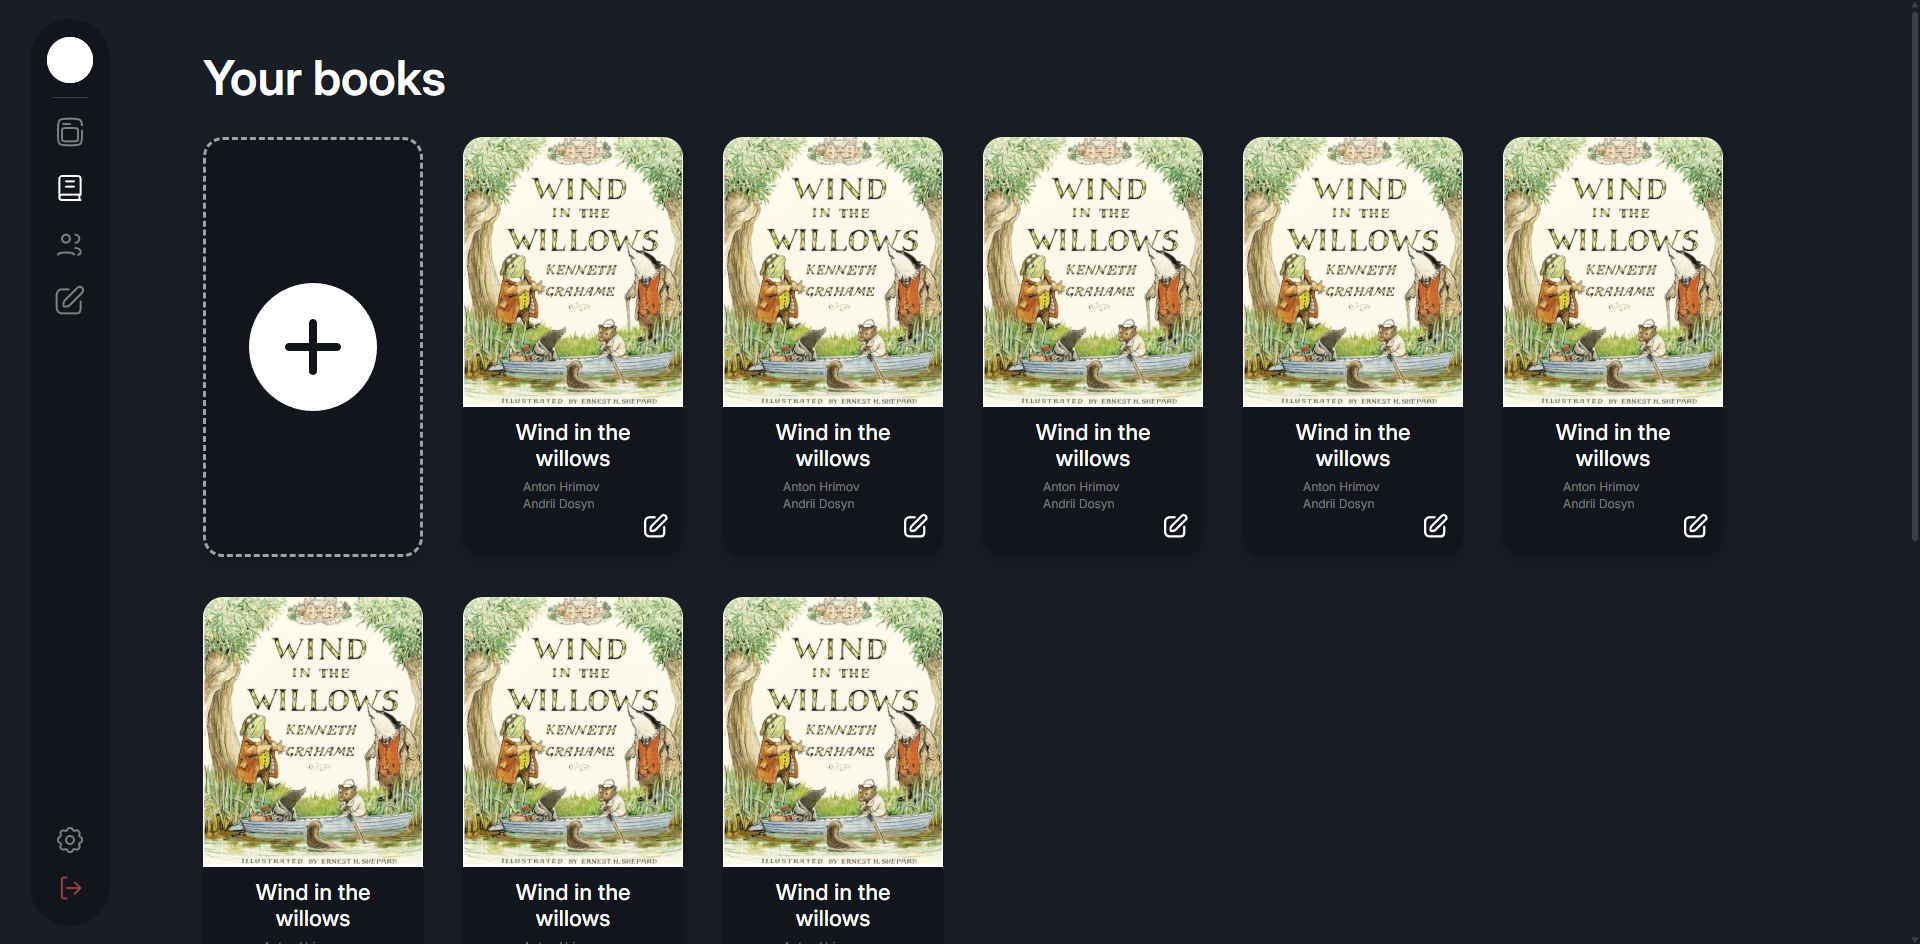
\includegraphics[scale=0.23]{library.png}
\end{figure}
\begin{figure}[H]
\centering
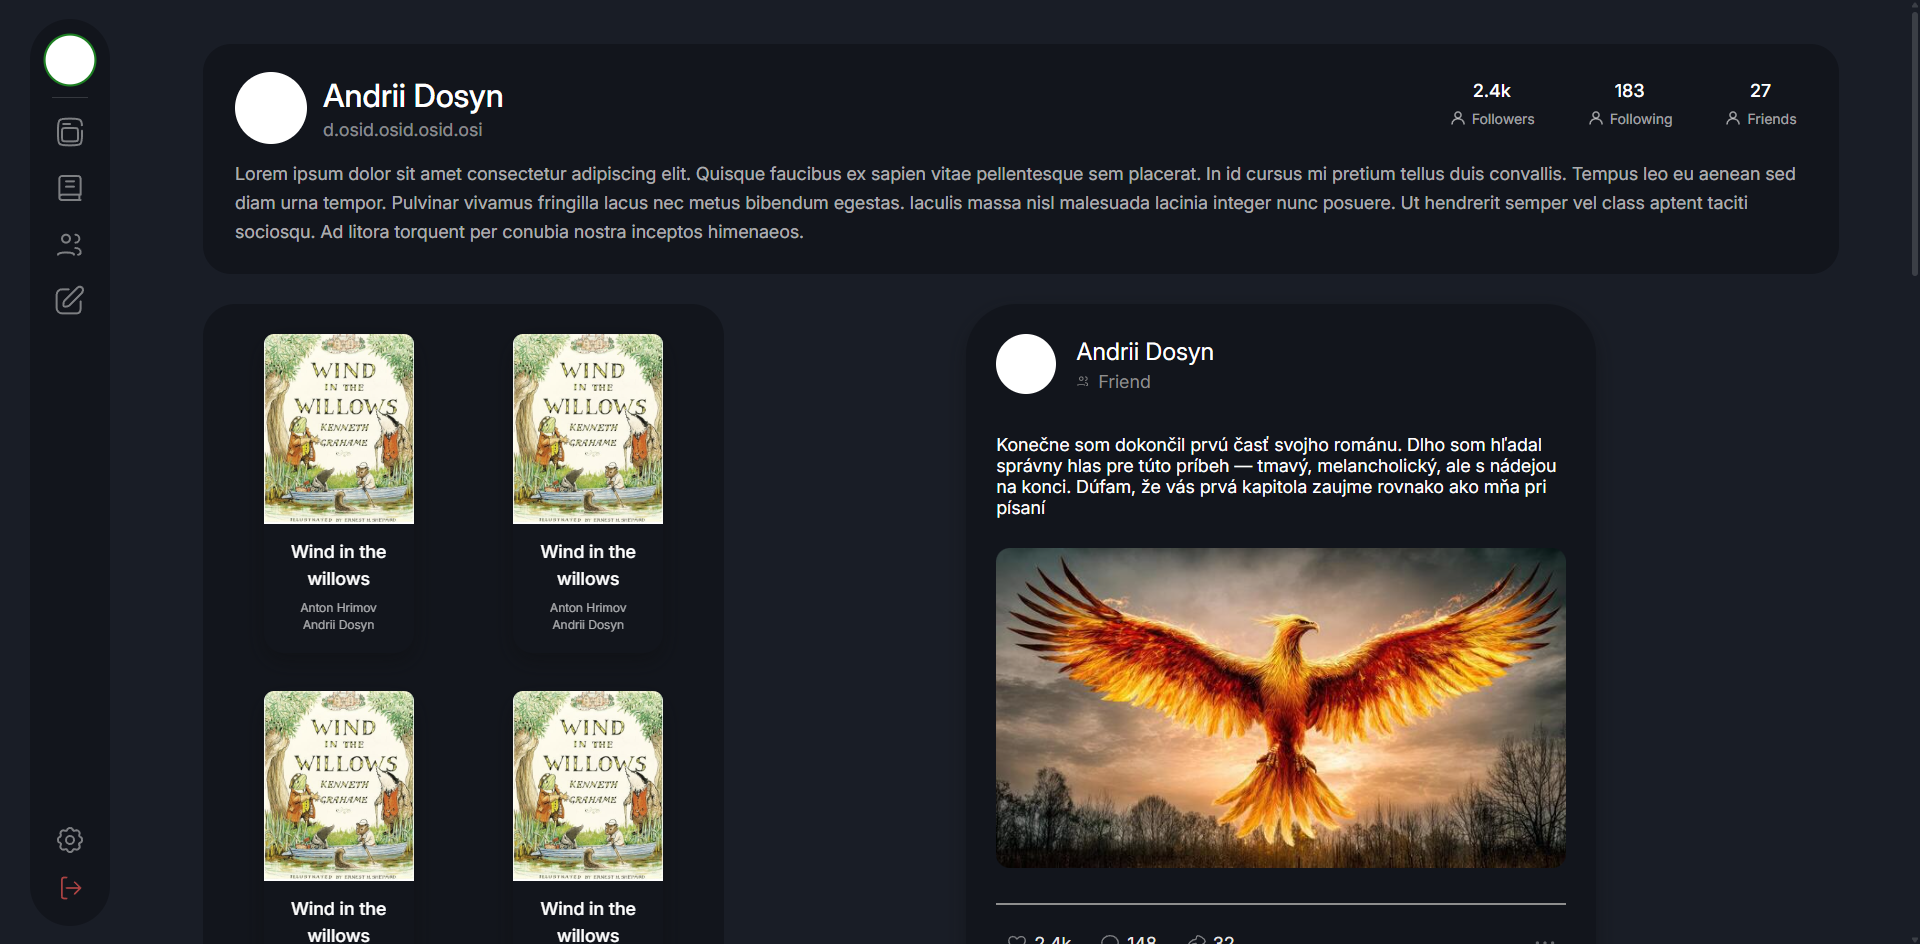
\includegraphics[scale=0.23]{profile.png}
\end{figure}
Profil zhromažďuje autorove informácie, zatiaľ čo Library slúži na správu rozpracovaných kníh.

\subsection{Detail knihy a Príspevku}

\begin{figure}[H]
\centering
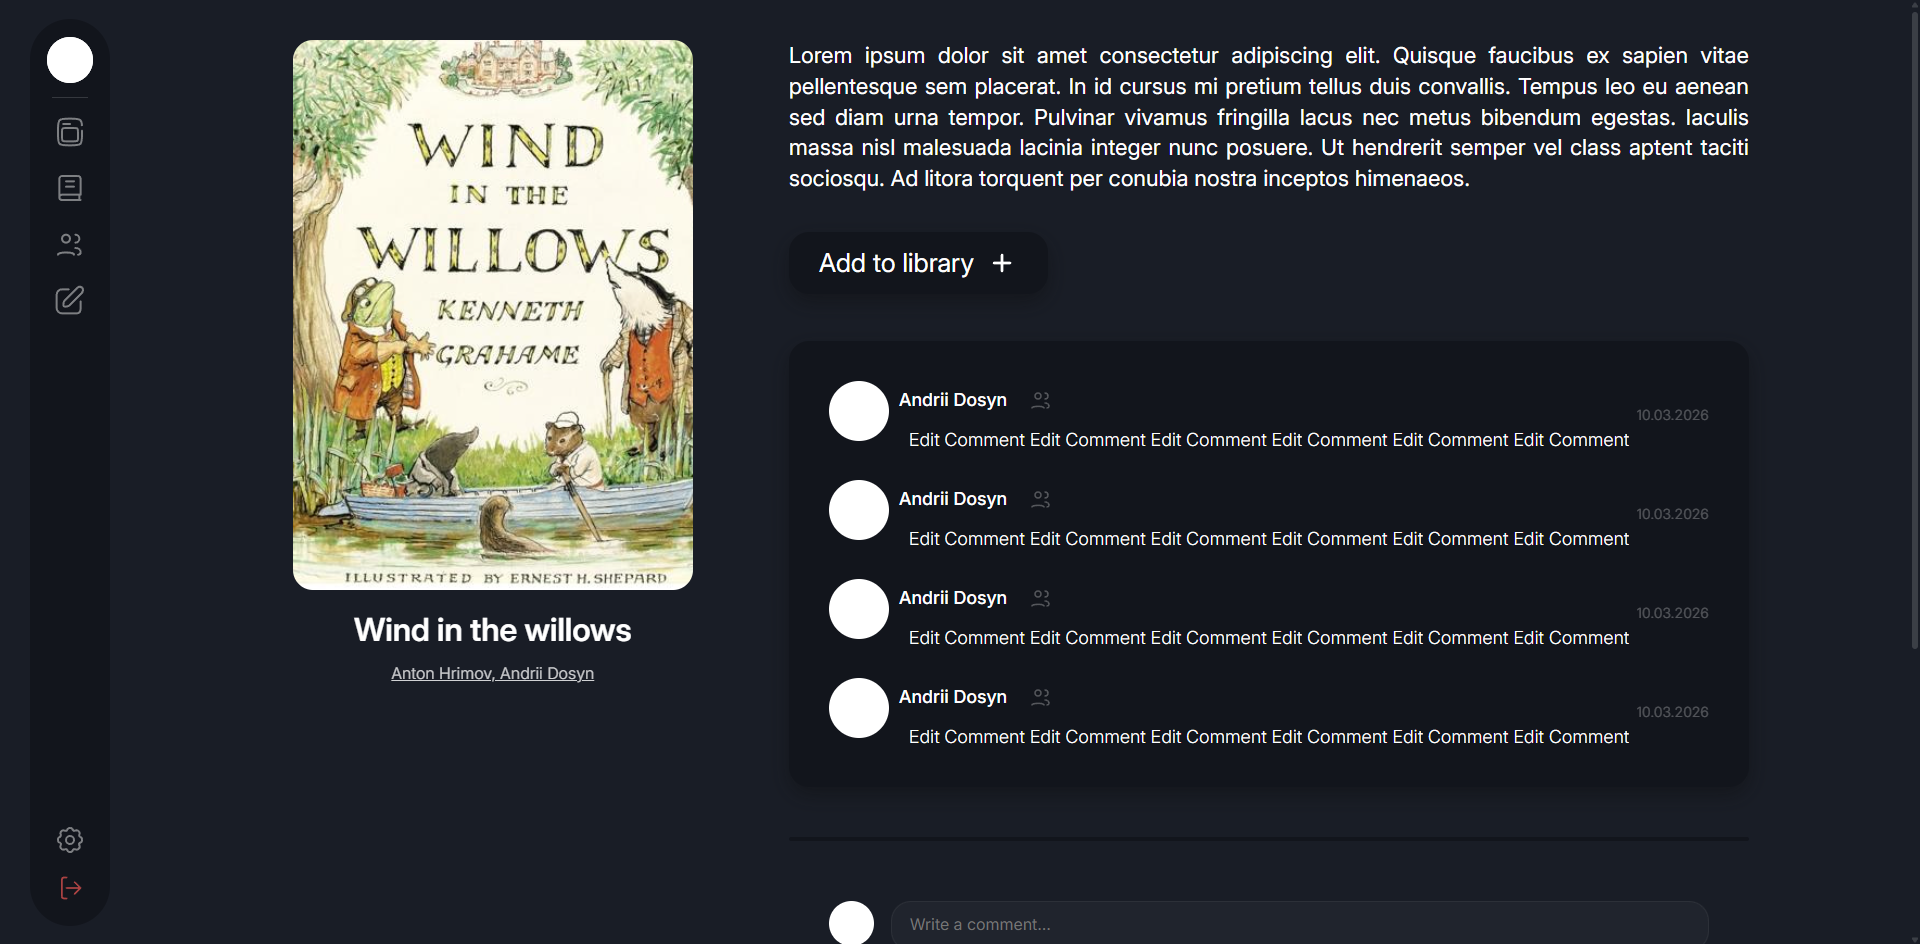
\includegraphics[scale=0.23]{book_page.png}
\end{figure}
\begin{figure}[H]
\centering
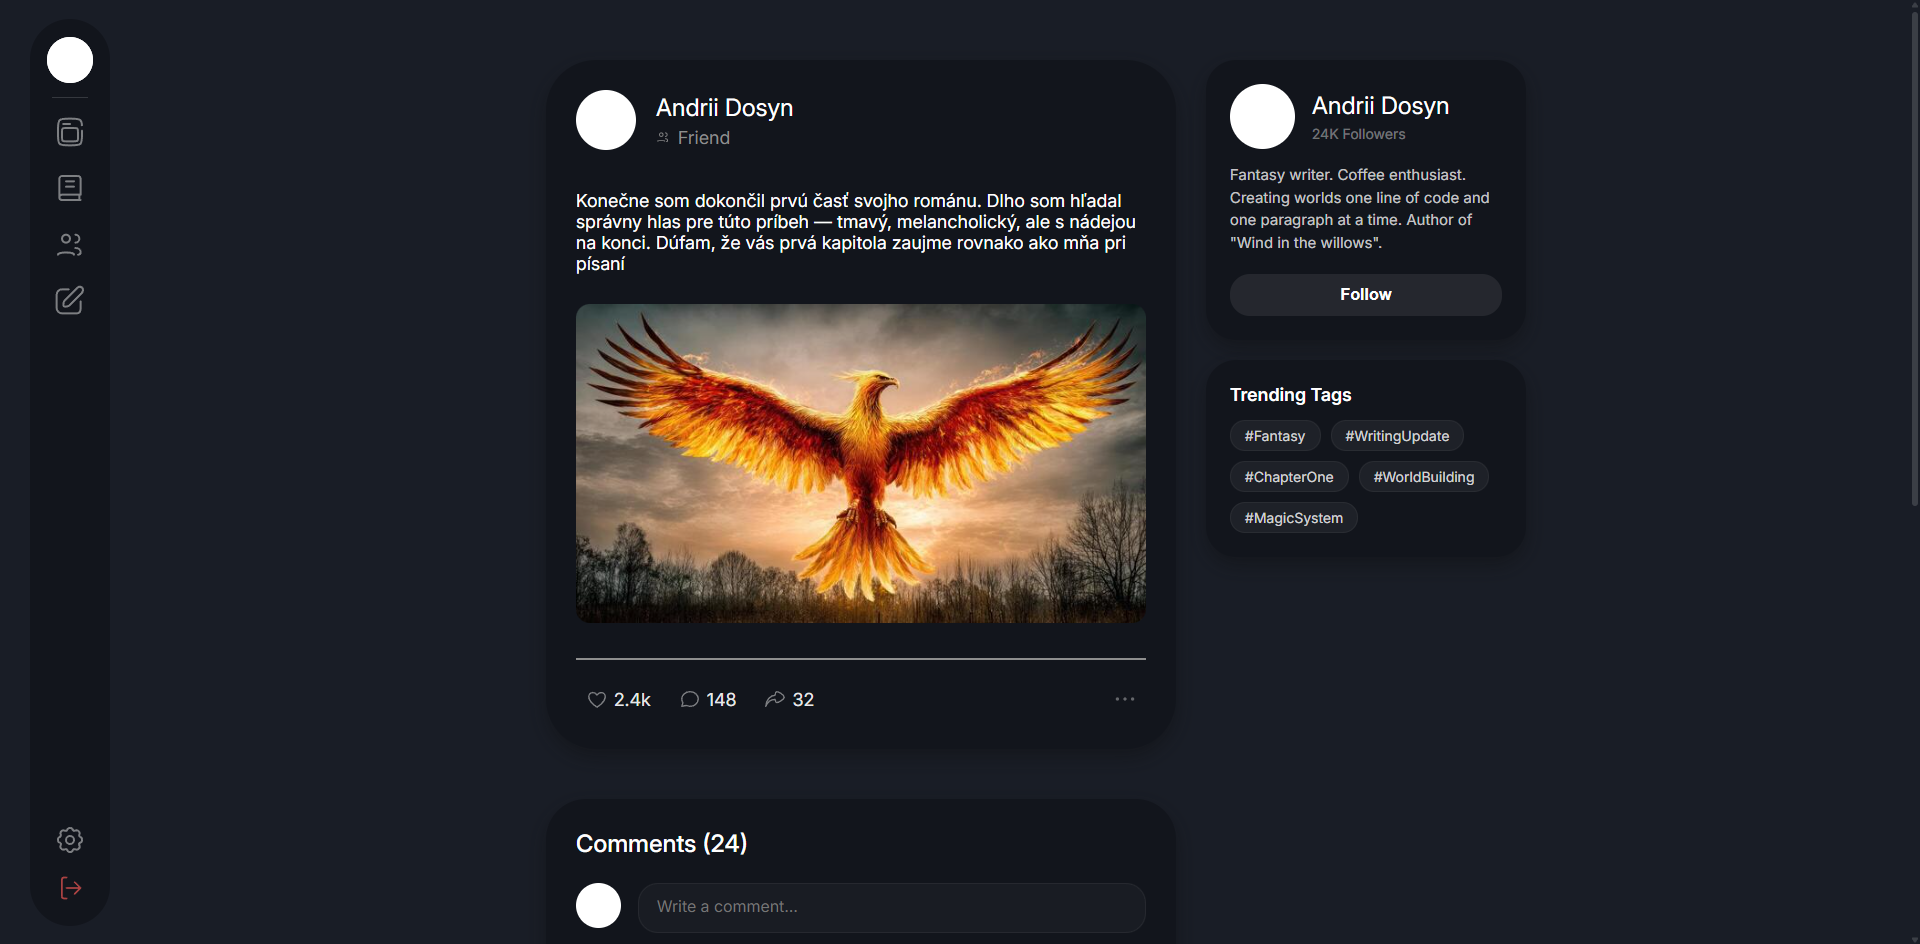
\includegraphics[scale=0.23]{post_page.png}
\end{figure}
Stránky využívajú prepracovaný dvojstĺpcový dizajn a implementujú pokročilú stromovú štruktúru komentárov.

\subsection{Pokročilý editor a edit requests}

\begin{figure}[H]
\centering
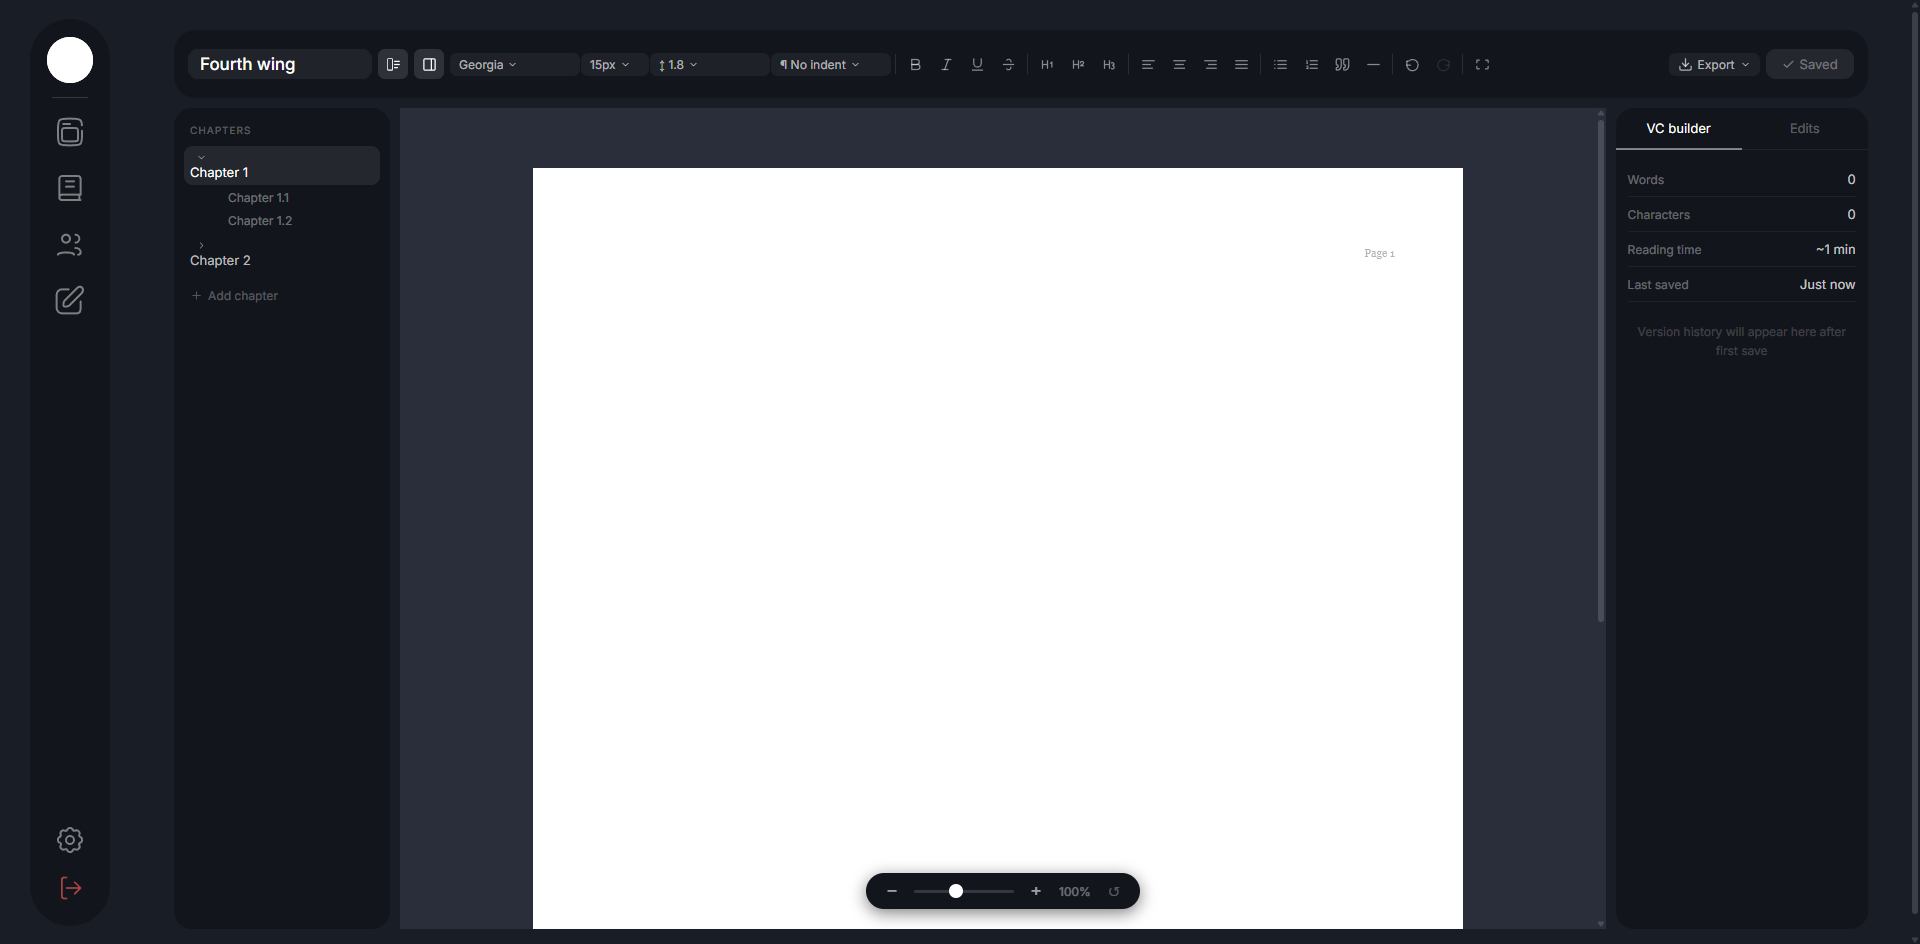
\includegraphics[scale=0.23]{editor.png}
\end{figure}
\begin{figure}[H]
\centering
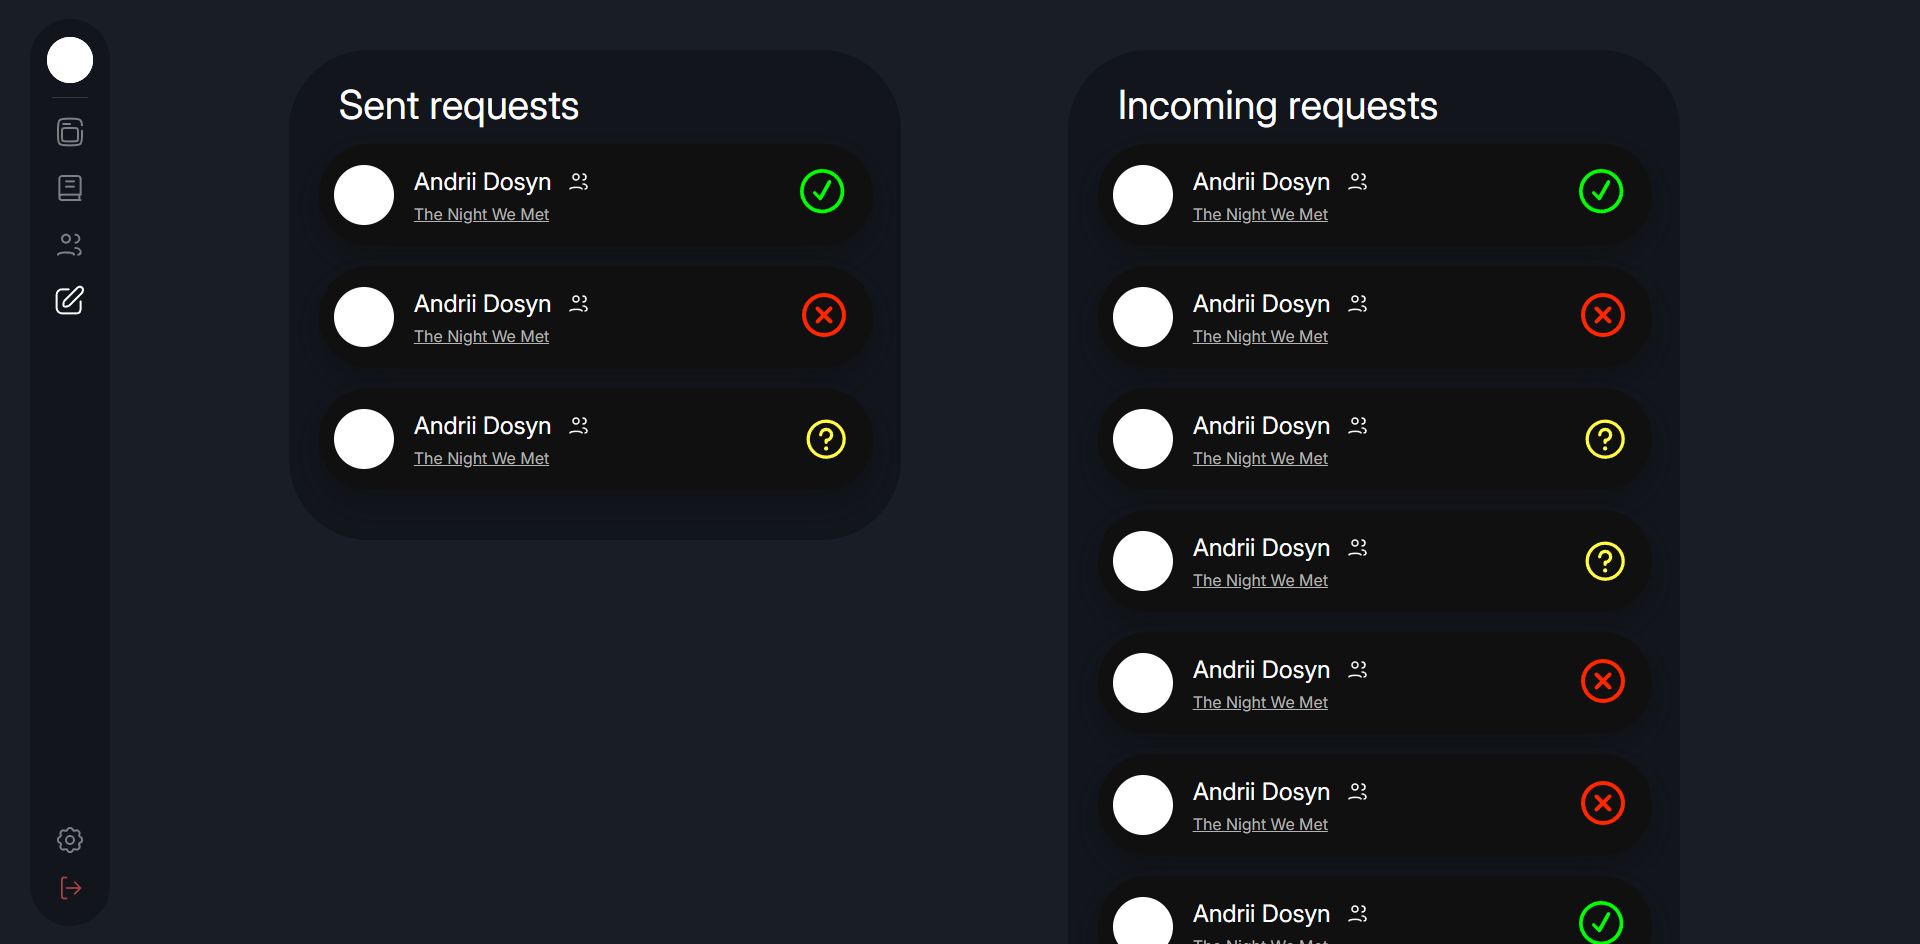
\includegraphics[scale=0.23]{edit_requests.png}
\end{figure}
Súčasťou platformy je profesionálny editor stránkovaný na vizuálny formát A4 (Focus mode). Autori tu spravujú návrhy na úpravu od čitateľov.

\newpage

\section{Používateľský manuál – Ako spustiť program}

Z dôvodu optimalizácie veľkosti repozitára nie sú na GitHube zaradené inštalované knižnice a systémové moduly (\texttt{node\_modules}, Python virtual env). Služby je potrebné pred prvým spustením zinicializovať oddelene:

\textbf{1. Frontend používateľské rozhranie (React)} \\
Pre úspešné spustenie je nutné mať v systéme nainštalované prostredie \textbf{Node.js} (aspoň verziu 18). Architektúra klienta stavia na modernom build-systéme \textbf{Vite} a aktívne predinštalováva pokročilé knižnice (ako \texttt{react-router-dom} na smerovanie, \texttt{axios} pre API, textový balík \texttt{tiptap} a nástroje na PDF export ako \texttt{jspdf}). Nasmerujte terminál do priečinka \texttt{/frontend}. Najskôr nainštalujte závislosti s použitím Node balíčkovača a následne spustite lokálny dev-server cez \textbf{Vite}.
\begin{itemize}
    \item \texttt{npm install} (doinštaluje závislosti z \texttt{package.json} nad repozitárom)
    \item \texttt{npm run dev} (zapne platformu cez bleskový Vite server)
\end{itemize}

\textbf{2. Asynchrónna AI Mikroslužba (Zadanie2\_fixed)} \\
Pracovný Python backend beží nad balíkom FastAPI. Prejdite terminálom do koreňa Python mikroslužby a zavolajte:
\begin{itemize}
    \item \texttt{pip install -r requirements.txt} (stiahnutie knižníc vrátane \texttt{spaCy})
    \item \texttt{python -m spacy download en\_core\_web\_sm} (povinný sťahovač en modelov)
    \item \texttt{uvicorn main:app --reload} (finálne lokálne spustenie servera)
\end{itemize}
Pre úspešné prepojenie sa predpokladá, že súčasne bežíte aj jaderný Spring Boot modul.

\section{Záver}

Úspešná integrácia rozsiahlej Spring Boot infraštruktúry spoločne z Python AI analytickým modulom vytvorila silný predpoklad pre funkčnú sociálnu sieť pre autorov a čitateľov. Aplikovaním overených OOP princípov sa ukázala pripravenosť architektúry na ďalšie škálovanie, pridávanie nových perzistentných vrstiev a pokročilé napájania na umelú inteligenciu. Dátový model bezpečne pracuje so vzťahmi nad databázami a vizuálna ukážka odráža progres naplnenia základnej používateľskej cesty definovanej na začiatku projektu.

\end{document}